\documentclass[handout]{beamer}
\usepackage[frenchb]{babel}
\usepackage[T1]{fontenc}
\usepackage[utf8]{inputenc}
\usepackage{graphicx}


% functions to plot
\def\func(#1){(#1)*(1-(#1))}
\hypersetup{colorlinks = true,linkcolor = blue,urlcolor  = blue}
            
\newcommand{\qGraph}[1]{\begin{center} \includegraphics[width =
\textwidth]{#1}\end{center}}

\newcommand{\mcl}{\mathcal}


\newenvironment{iPar}[1]{\textbf{#1} \begin{itemize}}{\end{itemize}}

\newcommand{\inc}{{inc}}
\newcommand{\cp}{{cmp}}
\newcommand{\bull}{$\bullet\;$} 

\newcommand{\esp}{\mathbf{E}} \newcommand{\ul}[1]{\underline{#1}}
\newcommand{\ol}[1]{\overline{#1}} \newcommand{\ora}[1]{\textbf{#1}}
\newcommand{\wh}{\widehat}
\newcommand{\mdp}{\medskip \pause}
\newcommand{\mc}{\mathcal}

\title{Échange et Prix}
\author{Microéconomie \\ 20851}
\date{}

\begin{document}

\frame{\titlepage}

\section[Outline]{}
\frame{\tableofcontents}

\section{}


\begin{frame}\frametitle{Itinéraire}

\begin{iPar}{Jusqu'à maintenant}
\item Choix du consommateur
\item Effets prix et richesse
\item Risque et temps
\item Mesurer le bien-être
\end{iPar}\mdp

\begin{iPar}{Ce cours: échange}
\item Équilibre de marché en situation d'échange
\end{iPar}\mdp

\begin{iPar}{Plus tard}
\item  La production des firmes
\item Le comportement stratégique des firmes
\end{iPar}


\end{frame}

\section{Équilibre de marché}

\begin{frame}\frametitle{Économie d'échange}

\begin{iPar}{Contexte} \item Considérons une situation avec 2 consommateurs (1 et
2) et deux biens ($X$ et $Y$) \item Fonctions d'utilité $U_1(X,Y)$ et
$U_2(X,Y)$ \item Chaque consommateur a une dotation des deux biens, $B_1^e = (X_1^e,Y_1^e)$ et $B_2^e = (X_2^e,Y_2^e)$. \end{iPar}
\mdp


\begin{iPar}{Exemples} \item 2 fermiers, F1 qui a une dotation de patates, F2 qui a une dotation de bétail. \item  Deux pays: pays 1
avec une dotation de pétrole, pays 2 qui a une dotation de machineries \item D'où viennent ces dotations ? Nature (ressources) ou production
(bien de consommation, machinerie ...). Nous en reparlerons avec la production. 
\end{iPar}

\end{frame}

\begin{frame}\frametitle{Équilibre de marché}

\begin{iPar}{Demande individuelle} \item Consommateur 1 choisit consommation
$(X_1^c, Y_1^c)$  \item Étant donné les prix $p_X$ et $p_Y$, contrainte budgétaire est $$  p_X X_1^c + p_Y Y_1^c  =  p_X X_1^e + p_Y Y_1^e$$
\item Les prix seront déterminés à l'équilibre.
\end{iPar}\mdp

\begin{iPar}{Normalisation}
\item  Deux prix inconnus $p_X$ et $p_Y$. Seulement les prix relatifs sont importants: contrainte budgétaire peut s'écrire $$
X_1^c + \frac{p_Y}{p_X} Y_1^c  =   X_1^e + \frac{p_Y}{p_X} Y_1^e$$
\item Définissons le prix relatif  $p = p_Y/p_X$  \end{iPar}
\end{frame}

\begin{frame} \frametitle{Équilibre de marché -- II}

\begin{iPar}{Définition} \item Demande individuelle:  $ \max U_1$ sous la contrainte  $ X_1^c + p Y_1^c  =   X_1^e + p Y_1^e$
\item On obtient $X_1^c(p)$ et $Y_1^c(p)$
\item  $p^*$ est un prix d'équilibre seulement si à
$p^*$, la demande est égale à l'offre $$X_1^c(p^*)+X_2^c(p^*) = X_1^e + X_2^e \quad
et \quad Y_1^c(p^*)+Y_2^c(p^*) = Y_1^e + Y_2^e  $$ \item $X_1^c(p^*) -
X_1^e =X_2^e - X_2^c(p^*)  \;$  est le montant de $X$ échangé  \item si $X_1^c - X_1^e < 0$, consommateur 1 est un offreur net de $X$.\end{iPar}\end{frame}


\begin{frame}{Hypothèses importantes}
\begin{itemize} \item Marché compétitif
les consommateurs sont \textbf{prenneurs de prix} \item Chaque bien vendu est homogène (pareil) et perçu de la même façon par le vendeur et l'acheteur \item Utilité du consommateur 1 ne dépend pas des actions de l'autre consommateur: \textbf{aucune externalité} \end{itemize} \end{frame}



\begin{frame}\frametitle{Un exemple} \begin{iPar}{Contexte}\item $U_1(X,Y) =
U_2(X,Y) = \log X + \alpha \log Y$ \item Prix $p_X= 1$, $p_Y = p$.
\item Dotation $X_1^e, Y_1^e, X_2^e, Y_2^e$ \end{iPar} \mdp
\begin{iPar}{Équilibrium} \item Solution des demandes individuelles: $$X_1^c =
\frac{1}{1+\alpha}(X_1^e + p Y_1^e) \quad et \quad Y_1^c =
\frac{\alpha}{1+\alpha}\frac{X_1^e + p Y_1^e}{p} $$ \item Équilibre sur
marché pour $X$  \begin{equation*} X_1^c(p) + X_2^c(p) = X_1^e + X_2^e
\Rightarrow p = \alpha \frac{X_1^e + X_2^e}{Y_1^e + Y_2^e}
 \end{equation*} \item Voir que marché pour $Y$ est aussi en équilibre à $p$.\\\pause \textbf{Question:} une seule inconnue et deux équations?\end{iPar} \end{frame}

\begin{frame} \frametitle{Loi de Walras}

\begin{iPar}{Une inconnue mais deux équations} \item Aucun problème: $$\left.
\begin{array}{l} p \textrm{ équilibre le marché pour } X \\
\& \textrm{ contrainte budgétaire tient} \end{array}\right\}\Rightarrow
\textrm{marché pour } Y \textrm{ en équilibre}$$ \item Contrainte budgétaire: $$ X_1^c + p Y_1^c  =   X_1^e + p Y_1^e \quad et \quad
X_2^c + p Y_2^c  =   X_2^e + p Y_2^e$$ \pause Si on fait la somme des deux contraintes $$ [X_1^c + X_2^c] + p [Y_1^c + Y_2^c] = [X_1^e + X_2^e] + p
[Y_1^e + Y_2^e]$$ \pause Équilibre sur $X$  implique $$ p
[Y_1^c + Y_2^c]  = p [Y_1^e + Y_2^e] \Rightarrow  Y_1^c + Y_2^c = Y_1^e +
Y_2^e$$ \end{iPar}

\end{frame}

\begin{frame}\frametitle{Un exemple (fin)}

\begin{iPar}{Statique comparé} \item Comment $p$ varie avec $\alpha$
(importance du bien $Y$) et les quantités aggrégées de $X$ et $Y$ ?
\pause \item Si $\alpha$ $\nearrow$ alors $p=p_Y$ $\nearrow$: parce que offre total est fixe $Y$, quand demande $Y$ augmente prix doit ajusté pour garder en équilibre. \pause \item Si $Y_1^e + Y_2^e
\nearrow$ alors $p=p_Y$ $\searrow$: doit baisser prix pour vendre dotation. 
\pause \item Si $X_1^e + X_2^e \nearrow$ alors $p = p_Y$ $\nearrow$ puisque
bien $Y$ devient relativement rare comparé à $X$\end{iPar}

\end{frame}

\section{Allocation Efficace au sens de Pareto}

\begin{frame}\frametitle{La boîte de Edgeworth} 

\begin{itemize}
    \item On trace l'espace possible des allocations dans une boîte d'Edgeworth
    \item La dotation initiale est un point dans cet espace
\end{itemize}
 
\textbf{Exercice A}: Montrer la dotation $(x^e_1,y_1^e) = (50,20)$ et $(x^e_2,y_2^e)=(20,50)$ dans une boite d'Edgeworth.
\end{frame}


\begin{frame}\frametitle{Allocation efficiente au sens Pareto}
\begin{itemize}
    \item Un point dans la boîte d'Edgeworth où les courbes d'indifférence se croisent n'est pas un optimum de Pareto 
    \item On peut définir le noyau de référence pour ce point comme étant toutes les allocations qui sont une amélioration au sens de Pareto. 
    \item Quand le noyau est vide, on a une allocation efficiente au sens de Pareto : implique que les courbes d'indifférence sont tangentes.
    \item La courbe des contrats est la courbe qui identifie toutes les allocations efficiente au sens de Pareto. 
\end{itemize}

\end{frame}

\begin{frame}{Calcul d'un optimum}

On peut chercher à maximiser le bien-être d'un agent en prenant celui de l'autre fixe et en respectant les contraintes de ressources: 

\begin{eqnarray*}
\max_{X_1,Y_1,X_2,Y_2} u(X_1,Y_1) 
\end{eqnarray*}
sujet aux contraintes:
\begin{eqnarray*}
u(X_2,Y_2)\ge \overline{u}_2 \\
X_1 + X_2 \le X_e \\
Y_1 + Y_2 \le Y_e
\end{eqnarray*}

\end{frame}

\begin{frame}\frametitle{Quelques exercices} 


\textbf{Exercice B}: Trouvez l'allocation optimale pour des fonctions d'utilité $u_1$ et $u_2$ strictement positive et concave, $u_j = \sqrt{x_j y_j}$ pour les consommateurs $j=1,2$, à l'aide de la méthode du lagrangien.

\textbf{Exercice C}: Trouvez l'allocation optimale pour les fonctions d'utilité $u_j = \sqrt{x_j y_j}$ pour les consommateurs $j=1,2$ et des dotations totales de $x_e = 128$ et $y_e=32$ si $\overline{u}_2=48$.

\textbf{Exercice D}: Dans le cas de l'exercice C, est-ce que l'allocation $(64,28,64,4)$ est optimale? Si non, trouvez une amélioration qui est optimale dans le noyau. 

\end{frame}

\begin{frame}{Équilibre de marché dans la Boîte d'Edgeworth}
\begin{itemize}
    \item La contrainte budgétaire passe par les dotations et indique au prix $p$ les allocations possibles. 
    \item Un équilibre de marché implique que les $TMS$ sont égaux au rapport de prix.
\end{itemize}
\end{frame}

\begin{frame}\frametitle{L'échange meilleur que l'autarcie}

\begin{iPar}{Propriété:} \item Considérons $p^*$  prix d'équilibre et
$X^c_1 = X^c_1(p^*)$ et $Y^c_1 = Y^c_1(p^*)$ les quantités consommées par le consommateur 1\item On a $U_1(X^c_1, Y^c_1) \geq U_1(X^e_1, Y^e_1)$
\end{iPar}\mdp

\begin{iPar}{Pourquoi?} \item À $p^*$, le panier $B^e_1 = (X^e_1,Y^e_1)$ est disponible et le consommateur 1 choisit $B^c_1=(X^c_1, Y^c_1)$ \item Ceci implique que $U_1(X^c_1, Y^c_1) \geq U_1(X^e_1, Y^e_1)$
\pause \item Note: Si $U$ concave et $(X^c_1, Y^c_1) \neq (X^e_1,
Y^e_1)$ alors $U_1(X^c_1, Y^c_1) > U_1(X^e_1, Y^e_1)$ \end{iPar}

\end{frame}

\begin{frame}\frametitle{Propriété de l'équilibre de marché (I) -- 1er théorème du bien-être} \begin{iPar}{1er théorème du bien-être} \item  Un équilibre de marché est toujours un optimum de pareto. \item 
Une allocation est Pareto efficace si on ne peut pas améliorer le sort d'un consommateur sans nuire à celui d'un autre \end{iPar}\mdp



\begin{iPar}{Pourquoi?} \item<1-> Supposons aucune solution de coin (pas nécessaire mais simplifie) \item<2-> À l'allocation d'équilibre
$X^c_1(p^*),Y^c_1(p^*),X^c_2(p^*),Y^c_1(p^*)$ courbe d'indifférence du
consommateur 1 est tangent à la droite budgétaire, tangente à la courbe d'indifférence du consommateur 2 \item<3-> Ainsi, ceci implique que cette allocation est Pareto efficace.\end{iPar}

\end{frame}


\begin{frame}\frametitle{Le 2e théorème}

\begin{iPar}{Le 2e théorème du bien-être} \item En redistribuant les dotations, toute allocation de Pareto peut être obtenue comme équilibre de marché \item Requiert abilité de faire des taxes/paiements forfaitaires \item Souvent appelé une allocation décentralisée
\end{iPar}\mdp

\begin{iPar}{Pourquoi?}\item Supposons qu'il n'y a pas de solution de coin \item À n'importe quelle allocation $(X_1^*,Y_1^*)$ ( et valeur conséquente pour
$X_2^*,Y_2^*$) les courbes d'indifférences des deux consommateurs sont tangentes.
\item Considérons la ligne tangente. \item N'importe quelle dotation sur cette ligne résulte en un équilibre de marché $(X^*,Y^*)$. \end{iPar}

\textbf{Exercice E}: Trouvez les transfers de dotation et le prix, en partant de $(64,28,64,4)$ qui donne l'allocation optimale trouvé en D.  

\end{frame}


\begin{frame}\frametitle{Efficacité des marchés}
\begin{iPar}{Le 1er et 2e théorème établissent que} \item
Le marché est efficace \item Si par hasard on veut une autre allocation, on peut l'obtenir en redistribuant les ressources et en laissant les forces du marché fonctionner  \end{iPar}\mdp

\begin{iPar}{Résultat important: efficience décentralisée} \item Équilibre de marché requiert seulement que les agents connaissent leur propre préférence   \item Pas besoin du planificateur central qui connait toutes les préférences \item Donne naturellement un résultat optimal au sens de Pareto \item
Vision de Hayek: les marchés sont des aggrégateurs d'information \item L'économie planifiée perd cette information (et il est coûteux de trouver les préférences de chaque citoyen). 
\end{iPar}

\end{frame}

\begin{frame}\frametitle{Épilogue -- II -- limites}

\begin{iPar}{Les deux théorèmes sont intéressants mais reposent sur des hypothèses importantes} 
\item Marchés compétitifs (prenneur de prix) \item Les biens sont homogènes (on sait ce qu'on achète) \item Aucune externalité
\item On peut faire des taxes forfaitaires (pour 2e théorème)\end{iPar}\mdp

La théorie de l'équilibre général a eu un impact sur la profession: on n'a qu'à penser à la compréhension des marchés financiers, de la macroéconomie. 

\end{frame}

\begin{frame}\frametitle{Histoire de la théorie de l'équilibre général}

\begin{figure}
\centering
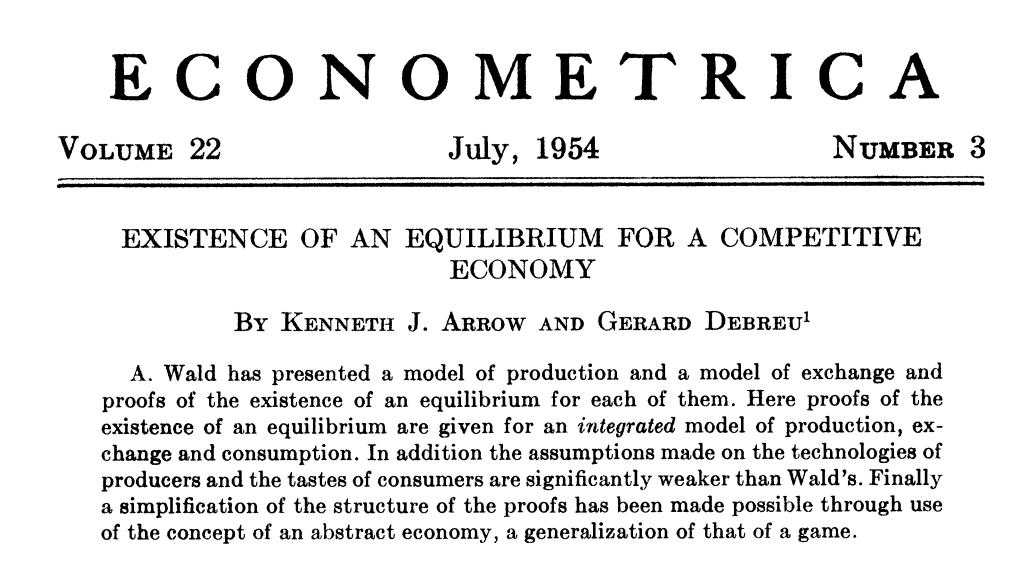
\includegraphics[scale=0.5]{ad1954.png}
\end{figure}

\end{frame}


\begin{frame}\frametitle{Histoire de la théorie de l'équilibre général}

Les deux venaient de background très différent (Arrow, économie), (Debreu, mathématique). Düppe (2017) raconte comment ce projet a vu le jour et a été réalisé.  

\begin{figure}
\centering

\includegraphics[scale=0.35]{invitation.png}
\caption{\href{https://www.cambridge.org/core/journals/journal-of-the-history-of-economic-thought/article/div-classtitlearrow-and-debreu-de-homogenizeddiv/761E76D5A52C948615066F502277D9DD}{Duppe (2017), Journal of History of Economic Thought}}
\end{figure}

\end{frame}

\end{document}




